
In our experiments, we evaluated our indexing techniques on two real world datasets. We have compared our indexing techniques by comparing the running time with that of the state of the art technique  . We are also concerned about the indexing time, especially for the M-tree index structure since we do not want our index procedure to run into hours.

The first dataset is the Swamidass dataset . The second dataset is from DUD, a directory of useful decoys for benchmarking virtual screening. DUD is provided by the Shoichet Laboratory in the Department of Pharmaceutical Chemistry at the University of California, San Francisco (UCSF). DUD is derived from ZINC, a database of commercially avaiilable compounds. To extarct fingerprints we used MOLPRINT2D, a molecular fingerprinting technique.


\section{M-tree based Indexing analysis}	

For these set of experiments the test bed used was a 4 Intel(R) Core(TM) i7-4770 CPU \@ 3.40GHz with 8GB RAM. We have varied several parameters in the experiment and have tried to estimate them emperically. We have used the non-binary version of the Swamidass dataset for all analysis of the M-tree. We use different dataset sizes of 1000, 10,000 and 100,000 number of chemical compounds.

For evaluation purposes we implemented a linear brute force scan to compute the range query and used that as a benchmark for the results. The result set obtained from our technique was compared with the linear brute scan answer set for verification purposes using the fingerprint id's. The query time and the indexing time is averaged over the 500 random query sample data points and the unit in ms per compound. We have varied the following parameters .


\subsection{Limiting Outlier Set Size }

\begin{figure}[ht]	
\centering
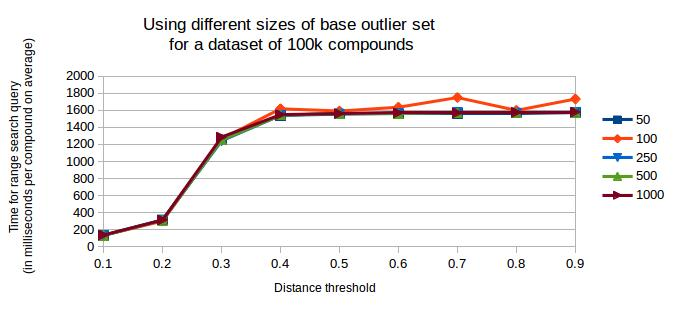
\includegraphics[width=1 \columnwidth]{img/image1.jpg}
\caption{M-tree: Average Range Query time versus Distance Threshold for various sizes of base outlier set}
\label{fig:5.1}
\end{figure}

Just to recap, it is the Minimum limiting size of the outlier set allowed (o). When the outlier set size falls below this limit, we terminate the indexing process.

As seen in \ref{fig:5.1} we can observe that the range search query time is almost constant with change in number of limiting outlier set size. We observed that the outlier base size did not have a significant effect on the query time for range search or on the number of comparisons. The indexing time increases with a lesser outlier base size because the depth of the M-tree increases . The algorithm is applied recursively on the outlier sets, hence when we have a lower base size limit for the outlier sets the number of times the recursion is applied is greater. Since we did not see a great change in query time or number of comparisons we have fixed the size the outlier size limit to 1/100th of the dataset size for all the future experiments.


\begin{figure}[ht!]	
\centering
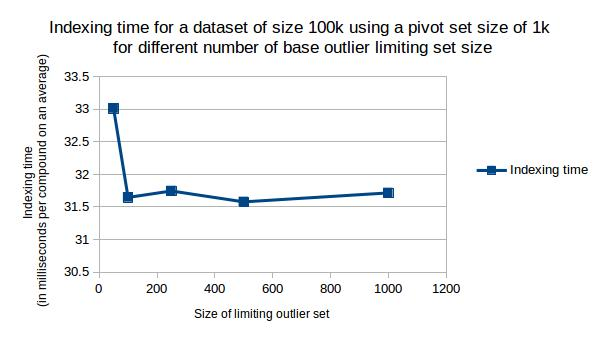
\includegraphics[width=1 \columnwidth]{img/image8.jpg}
\caption{M-tree: Indexing time versus different sizes of base limiting outlier set}
\label{fig:5.2}
\end{figure}


Ideally, indexing time should decrease with increase in number of limiting outlier size. This is because the depth of the M-tree grows with increase in the limitng size of the outlier set. The indexing process is a recursive procedure and termination occurs only when the size of the outlier set falls below the given limiting size. Hence in normal circumstances the indexing time must decrease as we increase the limiting size, but as seen in \autoref{fig:5.2} the decrease is minimal and changing \textit{o} doesn't change the indexing time much. 






\subsection{Pivot Set size}
The pivot set size as described earlier is the number of random pivots chosen at each step of the indexing process (p). \textit{p} determines the number of nodes at every level of the index structure. The number of nodes at each level is equal to p+1.

\autoref{fig:5.3},\autoref{fig:5.4},\autoref{fig:5.5}  show how the range search query time varies versus different distance threshold for different sizes of the pivot set for databases of size 1,000 , 10,000 and 100,000 compounds respectively. We can observe the time is almost similar at high threshold values for different number of pivots. For low theshold values we are succesfully able to prune away all many nodes using triangle inequality. 


\begin{figure}[ht!]	
\centering
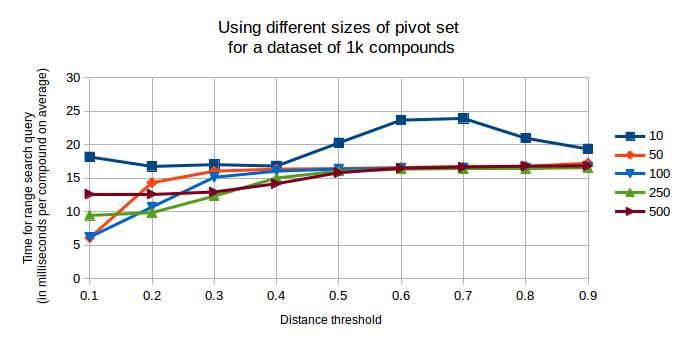
\includegraphics[width=1 \columnwidth]{img/image2.jpg}
\caption{M-tree: Average Range Query time versus Distance Threshold for various sizes of pivot set - 1k database}
\label{fig:5.3}
\end{figure}


\begin{figure}[ht!]	
\centering
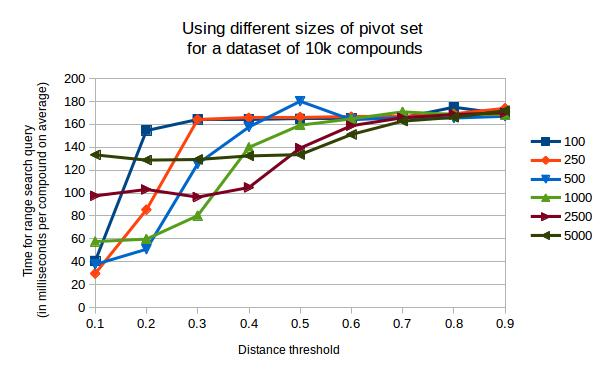
\includegraphics[width=1 \columnwidth]{img/image3.jpg}
\caption{M-tree: Average Range Query time versus Distance Threshold for various sizes of pivot set - 10k database}
\label{fig:5.4}
\end{figure}


\begin{figure}[ht!]	
\centering
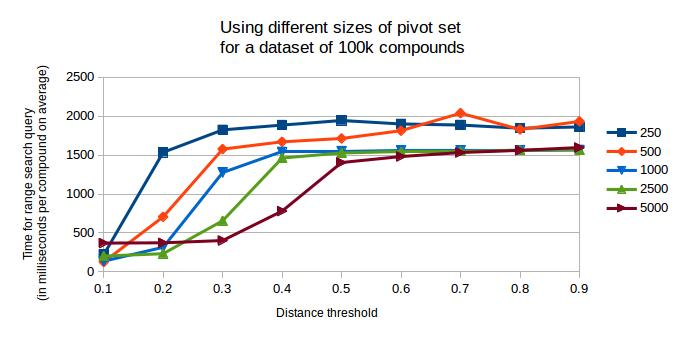
\includegraphics[width=1 \columnwidth]{img/image4.jpg}
\caption{M-tree: Average Range Query time versus Distance Threshold for various sizes of pivot set - 100k database}
\label{fig:5.5}
\end{figure}


We observe that indexing time is increasing almost linearly with increase in the number of pivots chosen at each step of the M-tree algorithm. Even though indexing is an offline process we do not want the indexing time to run into days. If indexing time is very high, updates to the chemical compound database would be very expensive since we need a re-indexing into the chemical database. Hence we need to have a threshold for indexing time.

\begin{figure}[ht!]	
\centering
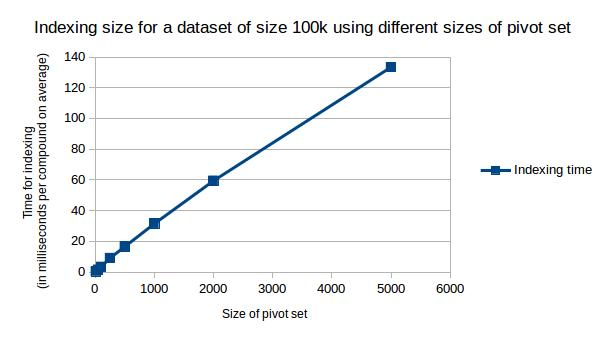
\includegraphics[width=1 \columnwidth]{img/image7.jpg}
\caption{M-tree: Indexing time versus different sizes of pivot set size}
\label{fig:5.6}
\end{figure}



\subsection{Threshold Distance}
As described in earlier sections, the range query distance threshold (t) is thse cutoff used for determining similarity. We observe that range search query time increases monotonically with threshold distance and begins to converge for higher values of threshold distance.  But this seems to hold true only if we use pivots above a particular threshold. 

There are two extremes here. If we use a very high number of pivots most of the time is spent doing computation involving triangle inequality bounds and hence it is not favourable. Similarly if we choose a very low number of pivots, it is not possible to exploit the bounds effectively to decisively prune or include the subtrees from our answer result set. For low number of pivots used we notice that for high and low values of threshold the query time is lower than that for the middle range, where bounds doesn't help well enough.


As seen in \ref{fig:5.7}, we observe that for low value of threshold at 0.1, the number of pivots to be chosen seems to have a minima between 500 and 1000 for a dataset size of 100k after which it increases . This is because there is a tradeoff between the time saved by pruning the subtrees versus the time utilized in checking if the nodes can be actually pruned.  For a high threshold value of 0.9 it can be seen that we require more number of pivots . 

\begin{figure}[ht!]	
\centering
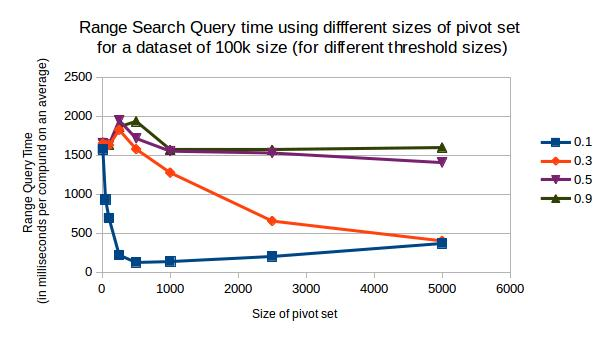
\includegraphics[width=1 \columnwidth]{img/image5.jpg}
\caption{M-tree: Average Range Query time versus various sizes of pivot set for different theshold distances}
\label{fig:5.7}
\end{figure}



\subsection{Dataset Size}
We varied the dataset size for the non-binary version of the Swamidass dataset to 1000, 10,000 and 100,000 and compared the indexing time as well as range search query time for various thresholds. 


\begin{figure}[ht!]	
\centering
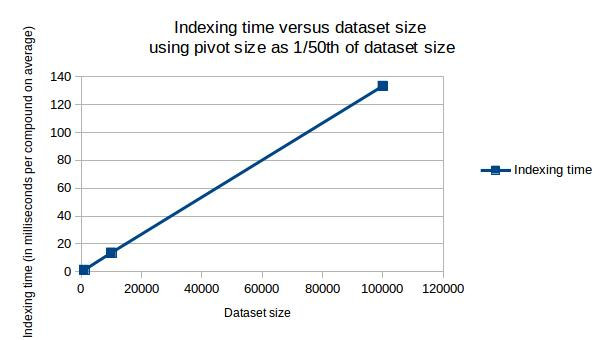
\includegraphics[width=1 \columnwidth]{img/image6.jpg}
\caption{M-tree: Indexing time versus dataset size}
\label{fig:5.8}
\end{figure}

\begin{figure}[ht!]	
\centering
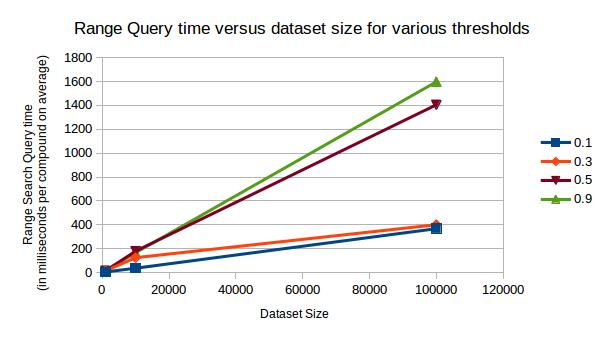
\includegraphics[width=1 \columnwidth]{img/image9.jpg}
\caption{M-tree: Range Query time versus dataset size}
\label{fig:5.9}
\end{figure}


As seen in \ref{fig:5.9}, we can observe that for a particular value of the distance threshold , the range search query time also increases linearly with dataset size . The slope is higher for higher values of threshold distance.

As seen in \ref{fig:5.8} we can observe that the average indexing time per compund on average increases linearly with increase in dataset size . This is as a result of our pivoting method with sampling which reduces the computation. If our pivoting step had been an exhaustive search on the database the curve would have not been linear, 





\section{Inverted Indexing Analysis}

For the below experiments the testbed used was a server with 512GB RAM, 24TB disk space, and 2 quad core Xeon processor. We tested the inverted index structure against both binary as well as non-binary versions of the Swamidass dataset. For evaluation and verification processes, a complete linear database scan was done as with the M-tree case to compare the result sets. One advantage of Inverted indexing procedure over the M-tree index structure is the much lesser time required for the indexing step. 

Indexing time per compound is observed to be almost constant between 1ms to 2ms per compound on average. As observed in \ref{fig:5I1} the graph is almost straight parallel to the x-axis for both the binary as well as the non-binary dataset.


\begin{figure}[ht]	
\centering
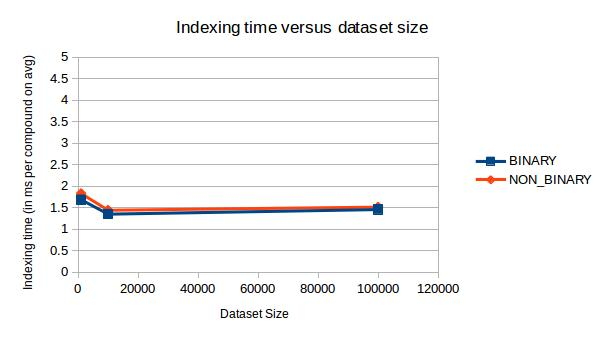
\includegraphics[width=1 \columnwidth]{img/imageI1.jpg}
\caption{Inverted Index: Indexing time versus dataset size for Inverted Indexing}
\label{fig:5I1}
\end{figure}


\begin{figure}[ht]	
\centering
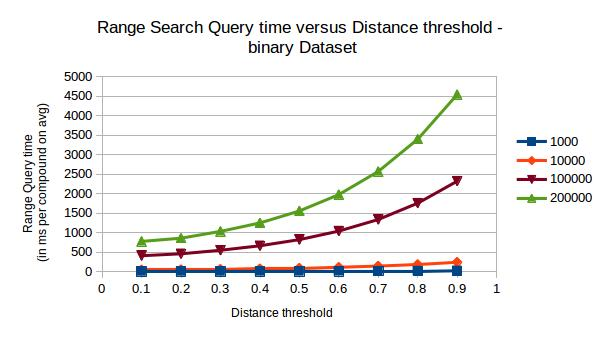
\includegraphics[width=1 \columnwidth]{img/imageI2.jpg}
\caption{Inverted Index: }
\label{fig:5I2}
\end{figure}

\begin{figure}[ht]	
\centering
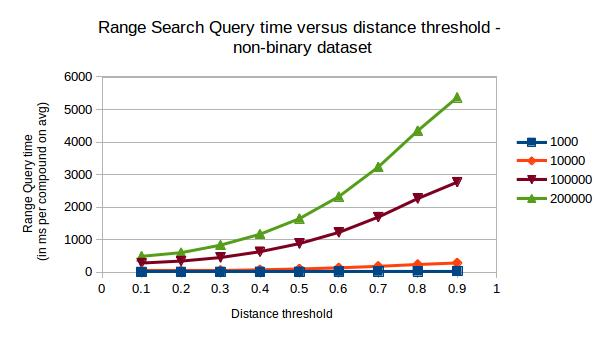
\includegraphics[width=1 \columnwidth]{img/imageI3.jpg}
\caption{Inverted Index: }
\label{fig:5I3}
\end{figure}




\section{Comparison of our techniques}





\begin{figure}[ht]	
\centering
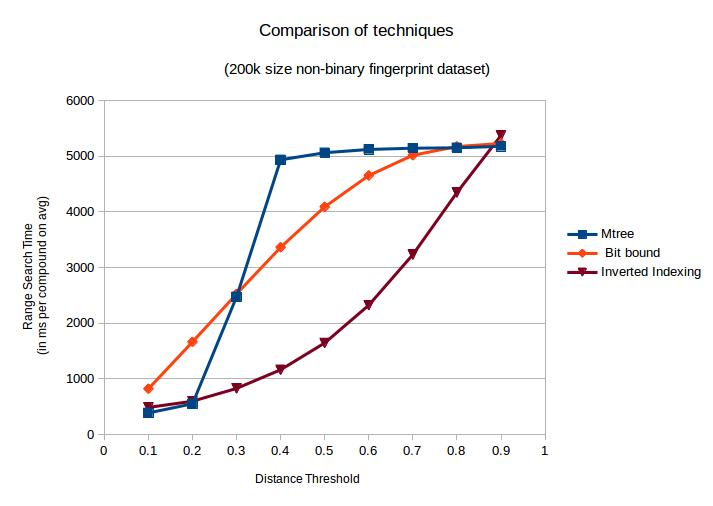
\includegraphics[width=1 \columnwidth]{img/imageC1.jpg}
\caption{Comparsion: }
\label{fig:5I1}
\end{figure}


\begin{figure}[ht]	
\centering
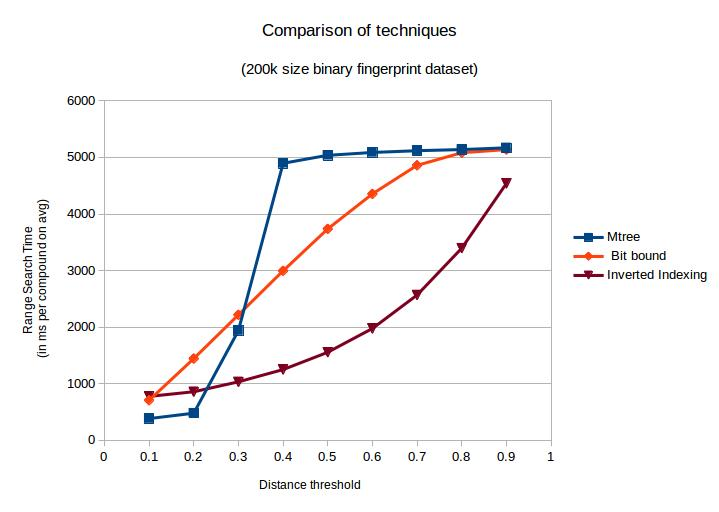
\includegraphics[width=1 \columnwidth]{img/imageC2.jpg}
\caption{Comparsion: }
\label{fig:5I2}
\end{figure}

\begin{figure}[ht]	
\centering
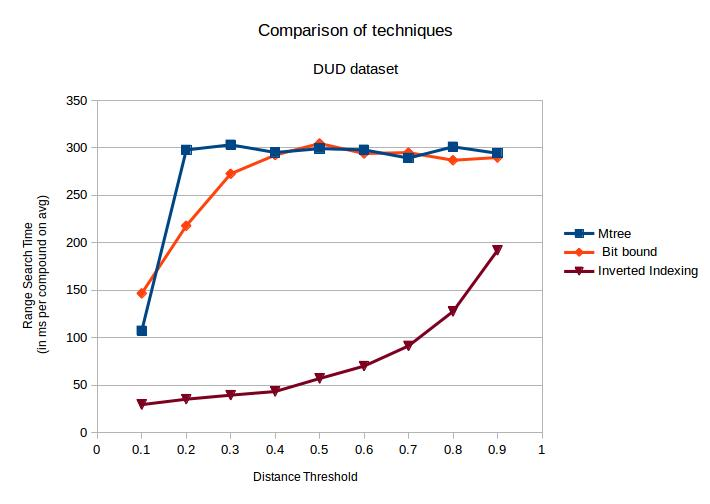
\includegraphics[width=1 \columnwidth]{img/imageC3.jpg}
\caption{Comparsion: }
\label{fig:5I3}
\end{figure}

